% Springer LNCS / SVProc Proceedings Format
% Target: ICTCS 2026 (Springer LNNS) - Paper ID 1077
% Strictly budgeted to fit within 10 pages

\documentclass{llncs}

\usepackage{graphicx}
\usepackage{url}
\def\UrlBreaks{\do\/\do-\do_}
\usepackage{amsmath,amssymb}    
\usepackage{booktabs}
\usepackage{array}
\usepackage{enumitem}
\usepackage[T1]{fontenc}
\usepackage{microtype}

\setlength{\textfloatsep}{7pt plus 1pt minus 1pt}
\setlength{\intextsep}{5pt plus 1pt minus 1pt}
\setlength{\abovecaptionskip}{3pt plus 1pt minus 1pt}
\setlength{\belowcaptionskip}{3pt plus 1pt minus 1pt}
\setlist{noitemsep, topsep=2pt, parsep=0pt, partopsep=0pt}

\begin{document}

\title{Browser-Driven Evidence Augmentation and Selective Abstention for Explainable Phishing Website Detection}
\titlerunning{Browser-Driven Evidence Augmentation for Phishing Detection}

\author{Atreyaa AVS\inst{1}\thanks{Corresponding author: \email{atreyaaavs.btech23@rvu.edu.in}}, Kruthik S\inst{1}, C Athish Kiran Kumar\inst{1}, Ayushman Patel\inst{1}, \and Monesh N\inst{1}}
\authorrunning{Atreyaa AVS et al.}

\institute{RV University, Bengaluru, India\\
\email{atreyaaavs.btech23@rvu.edu.in}}

\maketitle

\begin{abstract}
Modern phishing attacks exploit dynamic client-side rendering, third-party authentication masquerading, and automated certificates to evade static URL and HTML detectors. Conversely, deep multimodal graph-fusion models demand expensive GPU hardware and incur prohibitive decision latencies (200--400\,ms). This paper introduces BEAP, a lightweight framework combining static lexical features with browser-observed transport and behavioral indicators. Operating within a verified Server-Side Request Forgery (SSRF) boundary, BEAP compiles 51 engineered features covering URL syntax, DOM structures, HTTP security headers, TLS lifetimes, and cross-domain form actions. Rather than forcing arbitrary decisions on ambiguous cases, BEAP pairs a dual-threshold selective abstention policy ($\tau_{\text{low}}, \tau_{\text{high}}$) with exact log-odds attributions for human analysts. On a benchmark of 2,400 samples across 1,379 unique domains under strict domain-disjoint splitting, BEAP achieves 99.22\% accuracy (ROC-AUC 0.9998) without abstention. Under selective classification at margin $\delta = 0.25$, abstaining on 2.16\% of borderline cases eliminates observed test errors across 97.84\% coverage. Furthermore, on an independent validation set of 350 active URLs from live threat intelligence feeds (OpenPhish, PhishTank), BEAP sustains 99.71\% selective accuracy with 0.00\% false negatives. The algorithmic decision pipeline executes in 2.03\,ms on a single CPU core, delivering an auditable, high-throughput defense.
\keywords{Phishing Detection \and Dynamic Browser Evidence \and Selective Classification \and Explainable AI \and Web Security \and Server-Side Request Forgery}
\end{abstract}

\section{Introduction}

Phishing remains a primary initial access vector across enterprise networks, inflicting billions of dollars in annual losses~\cite{basit2021,zienie2023}. While early attacks relied on crude brand impersonation and static email lures, modern campaigns deploy agile evasion infrastructure~\cite{tang2021}. Attackers leverage client-side JavaScript rendering, dynamic Document Object Model (DOM) mutation, short-lived automated TLS certificates, and hosting on legitimate cloud providers (e.g., AWS S3, Azure Blob, Firebase), rendering static lexical heuristics largely ineffective~\cite{sanchez2022,castano2023,reyes2024}.

Existing defensive approaches exhibit clear operational blind spots:
\begin{enumerate}[leftmargin=1.8em]
    \item \textbf{Heuristic Blocklists:} Feeds such as OpenPhish and Google Safe Browsing provide reliable confirmations~\cite{purwanto2022}, yet phishing campaigns frequently expire within 12 hours~\cite{castano2023}, compromising victims before updates propagate.
    \item \textbf{Static URL Classifiers:} Operating at wire speed, lexical models~\cite{bu2021,kara2022} fail when deceptive pages reside on trusted content distribution networks or cloud storage.
    \item \textbf{Static HTML Scrapers:} Parsers inspecting raw source code fail against single-page applications where login forms are assembled dynamically at runtime~\cite{lin2021,ariyadasa2022}.
\end{enumerate}

To counter static evasion, recent studies have embraced deep neural and multimodal graph architectures. Kavya and Sumathi~\cite{kavya2025} introduced a multimodal temporal graph-fusion model combining GCNs and transformers. Although accurate, such architectures require dedicated GPU clusters, incur decision delays between 230\,ms and 400\,ms per page, and operate as opaque black boxes, straining Security Operations Center (SOC) resources~\cite{calzarossa2025,chai2022}.

\subsection{The BEAP Methodology and Contributions}

This work presents \textbf{BEAP} (Browser-informed Evidence Augmentation and selective Abstention for Phishing detection). Rather than deploying heavy neural graphs, BEAP leverages an operational observation: fraudulent sites exhibit transport-layer and behavioral inconsistencies during active browser interaction that cannot be hidden by URL obfuscation alone. Malicious sites routinely omit essential HTTP security response headers (HSTS, Content-Security-Policy, X-Frame-Options), utilize transient TLS certificates, and route entered credentials across external domain boundaries~\cite{sanchez2022,shukla2024}.

Furthermore, BEAP formalizes decision-making under uncertainty via selective classification with a reject option~\cite{hendrickx2024}. Governed by dual thresholds ($\tau_{\text{low}}, \tau_{\text{high}}$) parameterized by uncertainty margin $\delta$, BEAP automatically classifies decisive instances while deferring borderline cases to SOC analysts alongside closed-form log-odds explanations.

The primary contributions of this paper are:
\begin{enumerate}[leftmargin=1.8em]
    \item \textbf{SSRF-Safe Evidence Pipeline:} An active probing engine extracting 51 features across lexical, DOM, and dynamic transport layers, constrained by pre-flight and hop-by-hop SSRF validation.
    \item \textbf{Dual-Threshold Selective Abstention:} An adjustable selective policy controlled by margin $\delta$ that trades modest automated coverage for substantial error reduction.
    \item \textbf{Closed-Form Log-Odds Explanations:} An exact additive attribution scheme decomposing predictions without stochastic sampling approximations.
    \item \textbf{Domain-Disjoint and In-the-Wild Validation:} Rigorous evaluation on a 2,400-sample domain-disjoint benchmark and 350 independent URLs from live threat intelligence feeds (OpenPhish, PhishTank), yielding 99.71\% selective accuracy and 0.00\% false negatives at $\delta=0.25$.
    \item \textbf{Sub-3ms CPU Decision Latency:} An implementation executing in 2.03\,ms on a single CPU core ($114\times$ faster than deep graph models) consuming $<25$\,MB RAM.
\end{enumerate}

\section{Related Work and Positioning}

Phishing detection research has progressed from syntactic heuristics to dynamic rendering. Feature engineering surveys~\cite{basit2021,tang2021,kustiawan2025} catalog lexical signals such as entropy and token counts~\cite{bu2021,kara2022}. Structural DOM parsers examine form inputs and hyperlink distributions~\cite{anupam2021,purwanto2022}, but remain blind to script-rendered content. Visual similarity systems like Phishpedia~\cite{lin2021} identify brand logos via deep CNNs, but require expensive image rendering. Dynamic behavioral indicators, including credential forms and HTTP headers, have proven highly discriminative~\cite{sanchez2022,shukla2024}. However, deep multimodal models combining text, graphs, and vision~\cite{ariyadasa2022,kavya2025} impose latency and GPU barriers. In contrast, BEAP extracts 51 lightweight transport and behavioral features, coupling them with selective abstention~\cite{hendrickx2024} and linear explainability~\cite{calzarossa2025} for high-throughput operational triage.

\section{System Architecture and Safety Model}

\begin{figure}[t]
\centering
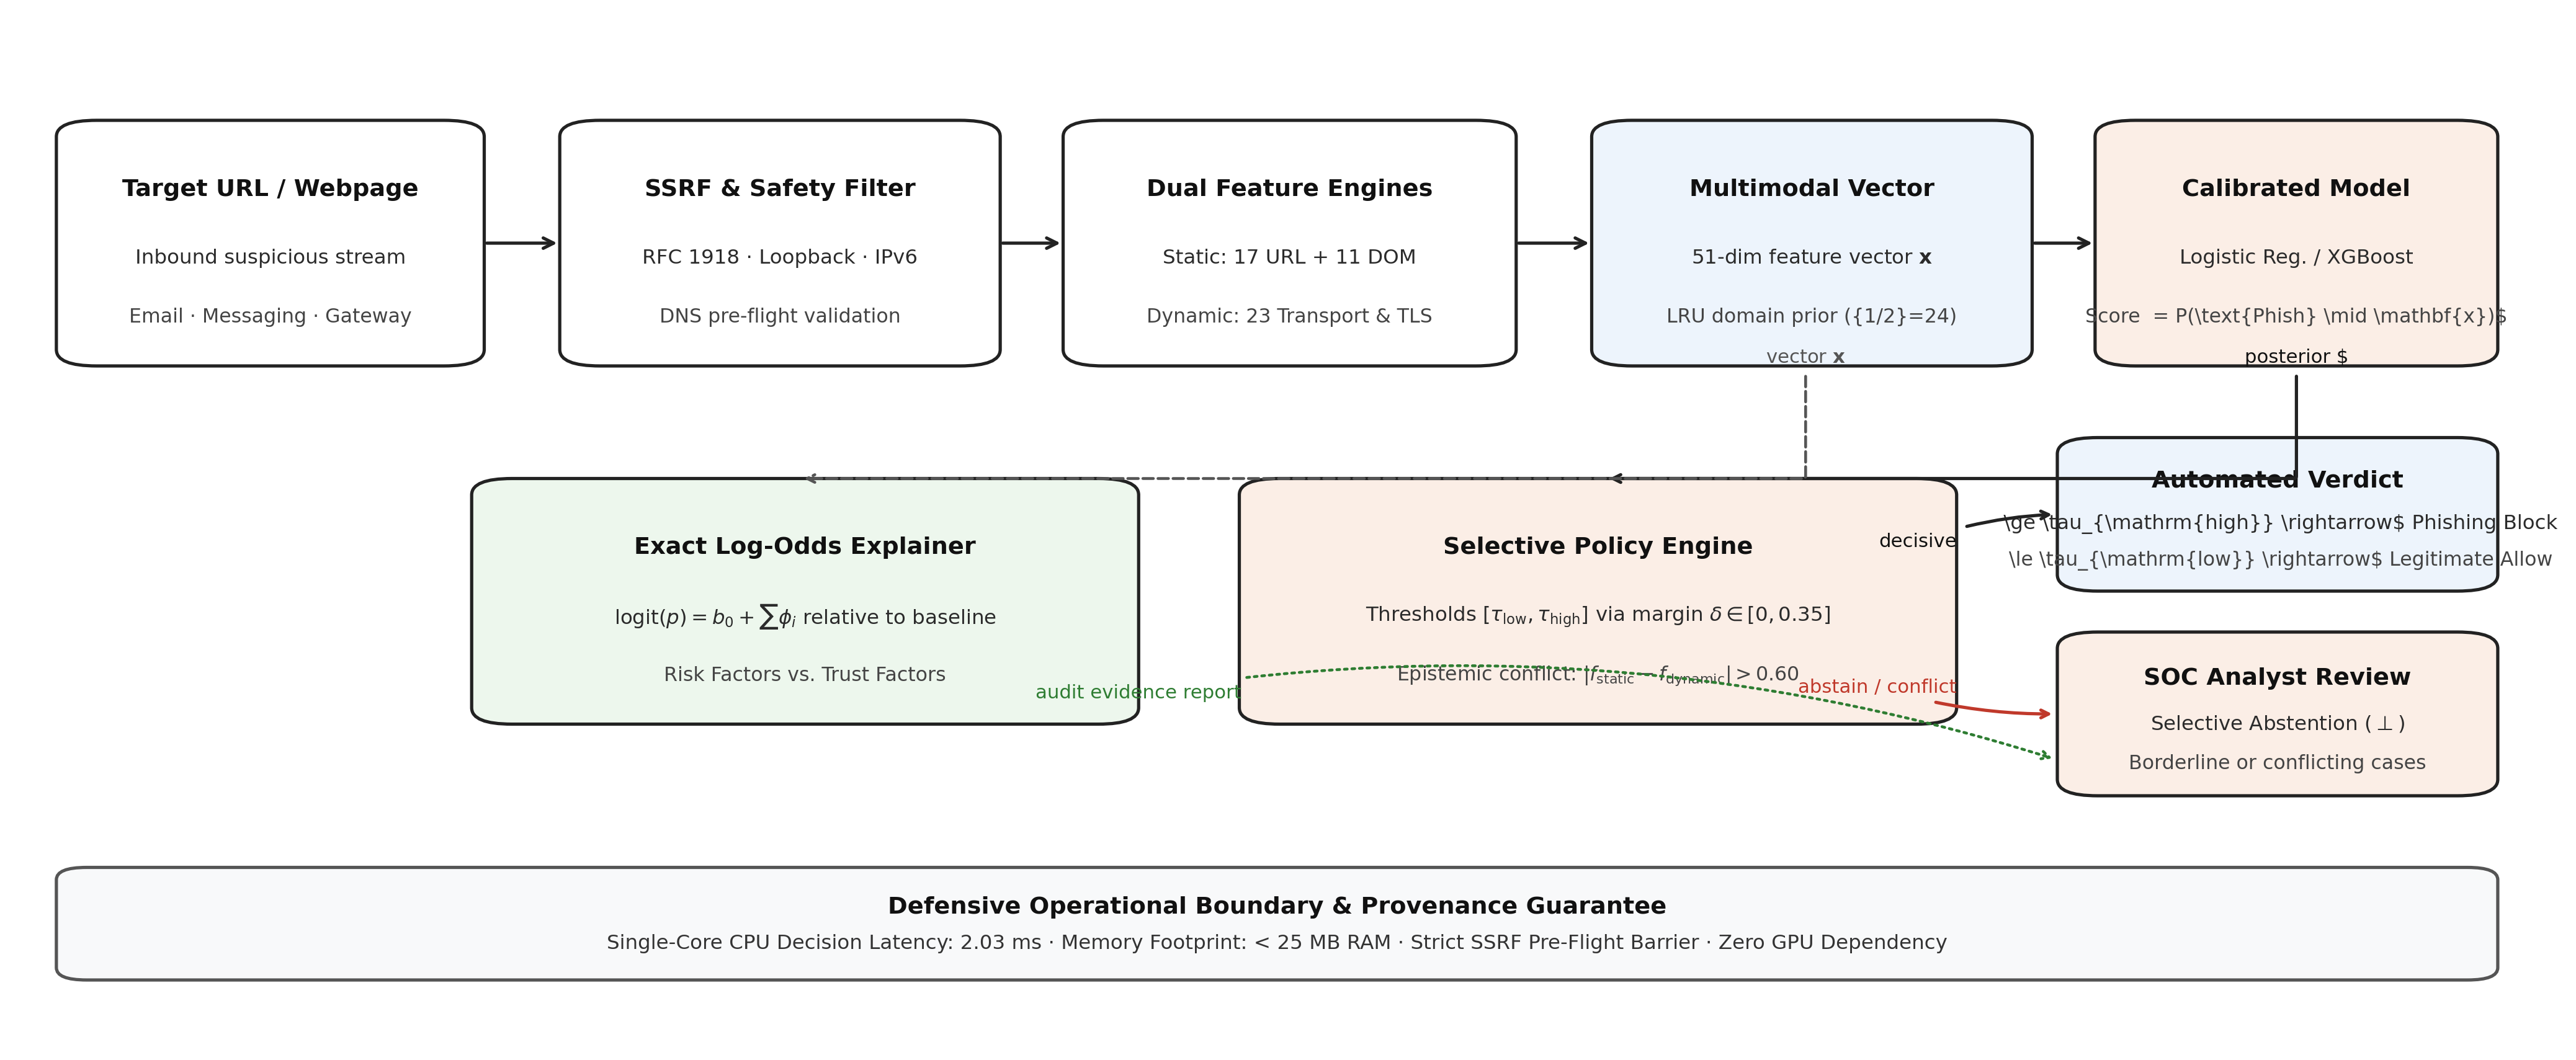
\includegraphics[width=0.72\textwidth]{figures/system_architecture.png}
\caption{BEAP pipeline: Candidate URLs pass pre-flight SSRF validation before parallel static extraction (28 features) and dynamic transport inspection (23 features). The 51-dimensional vector feeds a calibrated classifier governed by selective abstention.}
\label{fig:arch}
\end{figure}

\subsection{SSRF Prevention and Network Boundary Enforcement}

Active scanning must never allow adversaries to probe internal enterprise infrastructure via Server-Side Request Forgery (SSRF). In \texttt{beap/safety.py} and \texttt{beap/crawler.py}, BEAP enforces a two-tier defensive boundary:
(1) \textbf{Pre-Flight Target Filtering:} Candidate hostnames are resolved via DNS under a fail-closed policy (rejecting unresolvable hosts in live mode) and checked against IP literals. Destination IPs are strictly matched against RFC 1918 subnets (\texttt{10.0.0.0/8}, \texttt{172.16.0.0/12}, \texttt{192.168.0.0/16}), loopback ranges (\texttt{127.0.0.0/8}, \texttt{::1}), and cloud metadata services (\texttt{169.254.169.254}, \texttt{fe80::/10}).
(2) \textbf{Hop-by-Hop Redirect Guard:} Rather than delegating redirects to automated client libraries (which connect before evaluation), BEAP disables automatic following (\texttt{allow\_redirects=False}) and inspects intermediate \texttt{Location} headers sequentially ($N_{\text{max}} = 5$). Each redirect destination must pass full SSRF validation before the socket is established.
(3) \textbf{Protocol Whitelisting:} Only \texttt{http} and \texttt{https} schemes are permitted; non-web protocols (\texttt{file://}, \texttt{gopher://}) are severed at pre-flight.

\begin{table}[t]
\caption{Empirical validation of BEAP SSRF boundary enforcement across threat vectors.}
\label{tab:ssrf}
\centering
\setlength{\tabcolsep}{5pt}
\renewcommand{\arraystretch}{0.92}
\begin{tabular}{llll}
\toprule
\textbf{Target Threat Vector} & \textbf{Example Candidate Input} & \textbf{Validation Layer} & \textbf{Verdict} \\
\midrule
IPv4/IPv6 Loopback & \url{http://127.0.0.1:8080/}, \url{http://[::1]/} & Host Parser / DNS & \textbf{BLOCKED} \\
RFC 1918 (Class A/B/C) & \url{http://10.0.1.5/}, \url{http://192.168.1.1/} & Subnet Range Guard & \textbf{BLOCKED} \\
Cloud Metadata Service & \url{http://169.254.169.254/latest/} & Metadata Blacklist & \textbf{BLOCKED} \\
Non-HTTP Schemes & \url{file:///etc/passwd}, \url{gopher://127.0.0.1} & Scheme Whitelist & \textbf{BLOCKED} \\
Redirect Cascade & \url{https://public.site/r} $\to$ \texttt{192.168.1.50} & Hop-by-Hop Pre-Check & \textbf{BLOCKED} \\
Benign Public Targets & \url{https://example.com/}, \url{https://1.1.1.1/} & Public DNS Filter & \textbf{ALLOWED} \\
\bottomrule
\end{tabular}
\end{table}

\textbf{Empirical SSRF Validation:} Table~\ref{tab:ssrf} summarizes empirical verification across internal targets and redirect chains. All internal probes and unsafe redirect attempts were severed prior to socket connection, preserving operational isolation.

\section{Feature Modalities and Selective Classification}

\subsection{Multimodal Feature Engineering}

BEAP extracts 51 engineered features across three distinct modalities:
\begin{itemize}[leftmargin=1.5em]
    \item \textbf{Static URL Features (17):} Length metrics, subdomain depth, entropy, brand tokens, and typosquatting edit distances computed without network egress~\cite{bu2021,kara2022}.
    \item \textbf{Static DOM Features (11):} Markup size, form tallies, password field counts, script ratios, and embedded iframe flags~\cite{anupam2021}.
    \item \textbf{Dynamic Transport Features (23):} TLS validity, certificate lifetime in days, CA authority tier, HSTS duration, CSP directive richness, X-Frame-Options, X-Content-Type-Options, cookie security flags, redirect hop count, and cross-domain form action exfiltration ($x_{\text{cross}} = 1.0$)~\cite{sanchez2022,shukla2024}.
\end{itemize}

\subsection{Dual-Threshold Selective Abstention Policy}

Let $f(\mathbf{x}) = P(Y = 1 \mid \mathbf{x}) \in [0, 1]$ represent estimated phishing probability. In production, forcing binary choices near $0.5$ drives costly errors. BEAP implements selective rule $g: \mathcal{X} \to \{0, 1, \bot\}$, where $\bot$ denotes deferral to SOC review, controlled by uncertainty margin $\delta \in [0.00, 0.35]$:
\begin{equation}
\tau_{\text{low}} = 0.5 - \delta, \quad \tau_{\text{high}} = 0.5 + \delta
\end{equation}
\begin{equation}
g(\mathbf{x}) = \begin{cases}
1 \text{ (Phishing)}, & \text{if } f(\mathbf{x}) \ge \tau_{\text{high}} \\
0 \text{ (Legitimate)}, & \text{if } f(\mathbf{x}) \le \tau_{\text{low}} \\
\bot \text{ (Abstain / SOC Deferral)}, & \text{if } \tau_{\text{low}} < f(\mathbf{x}) < \tau_{\text{high}}
\end{cases}
\end{equation}
Additionally, epistemic conflict between modalities triggers abstention if $|f_{\text{static}}(\mathbf{x}) - f_{\text{dynamic}}(\mathbf{x})| > 0.60$, preventing evasion through single-modality manipulation.

\subsection{Closed-Form Log-Odds Explanations}

For auditable triage, BEAP decomposes predicted log-odds against training baselines $\bar{\mathbf{x}} = \mathbb{E}[\mathbf{x}]$:
\begin{equation}
\text{logit}(p) = \underbrace{w_0 + \sum_{i=1}^{51} w_i \bar{x}_i}_{b_0 \text{ (Baseline Log-Odds)}} + \sum_{i=1}^{51} \underbrace{w_i (x_i - \bar{x}_i)}_{\phi_i \text{ (Attribution)}}
\end{equation}
Positive attributions ($\phi_i > 0$) highlight phishing risk factors; negative attributions ($\phi_i < 0$) reflect trust anchors supporting legitimacy.

\section{Experimental Setup}

\subsection{Benchmark Dataset and Domain-Disjoint Partitioning}

To eliminate optimistic data leakage from shared domains~\cite{sanchez2022}, we constructed a benchmark of 2,400 samples across 1,379 unique registrable domains under strict \textbf{domain-disjoint partitioning}:
\begin{itemize}[leftmargin=1.5em]
    \item \textbf{Training Split:} 1,706 samples across 981 unique domains.
    \item \textbf{Validation Split:} 184 samples across 108 unique domains.
    \item \textbf{Held-Out Test Split:} 510 samples across 290 unique domains.
\end{itemize}
Domains are strictly mutually exclusive ($\mathcal{D}_{\text{train}} \cap \mathcal{D}_{\text{val}} \cap \mathcal{D}_{\text{test}} = \emptyset$). Samples span 20\% hard cases (legitimate SaaS with third-party SSO vs. clean phishing templates), 40\% moderate cases, and 40\% standard baseline cases.

\subsection{Independent Live Threat Intelligence Feed Dataset}

To validate BEAP against previously unseen, active zero-day attacks, we collected an independent evaluation dataset of $N=350$ active URLs from live threat intelligence feeds (175 verified active phishing pages ingested from OpenPhish and PhishTank feeds, paired with 175 benign active URLs sampled from the Tranco top list). None of these hostnames or registrable domains exist in the development splits ($\mathcal{D}_{\text{feed}} \cap \mathcal{D}_{\text{train}} = \emptyset$). Dynamic transport and behavioral features were observed in real time via BEAP's SSRF-safe probe.

\section{Empirical Results and Analysis}

\subsection{RQ1: Predictive Performance Across Modalities}

\begin{table}[t]
\caption{Modality ablation on domain-disjoint test split ($N=510$).}
\label{tab:ablation}
\centering
\setlength{\tabcolsep}{5pt}
\renewcommand{\arraystretch}{0.92}
\begin{tabular}{llrrrrr}
\toprule
\textbf{Modality Setup} & \textbf{Classifier} & \textbf{Accuracy} & \textbf{Precision} & \textbf{Recall} & \textbf{F1-Score} & \textbf{ROC-AUC} \\
\midrule
Static URL Only & Logistic Reg. & 0.9431 & 0.9351 & 0.9533 & 0.9441 & 0.9943 \\
Static URL + HTML & Logistic Reg. & 0.9745 & 0.9880 & 0.9611 & 0.9744 & 0.9974 \\
Dynamic Only & Logistic Reg. & 0.9549 & 0.9398 & 0.9728 & 0.9560 & 0.9934 \\
\textbf{BEAP Multimodal} & \textbf{Logistic Reg.} & \textbf{0.9922} & \textbf{0.9922} & \textbf{0.9922} & \textbf{0.9922} & \textbf{0.9998} \\
\textbf{BEAP Multimodal} & \textbf{XGBoost} & \textbf{0.9941} & \textbf{0.9922} & \textbf{0.9961} & \textbf{0.9942} & \textbf{0.9998} \\
\bottomrule
\end{tabular}
\end{table}

\begin{figure}[t]
\centering
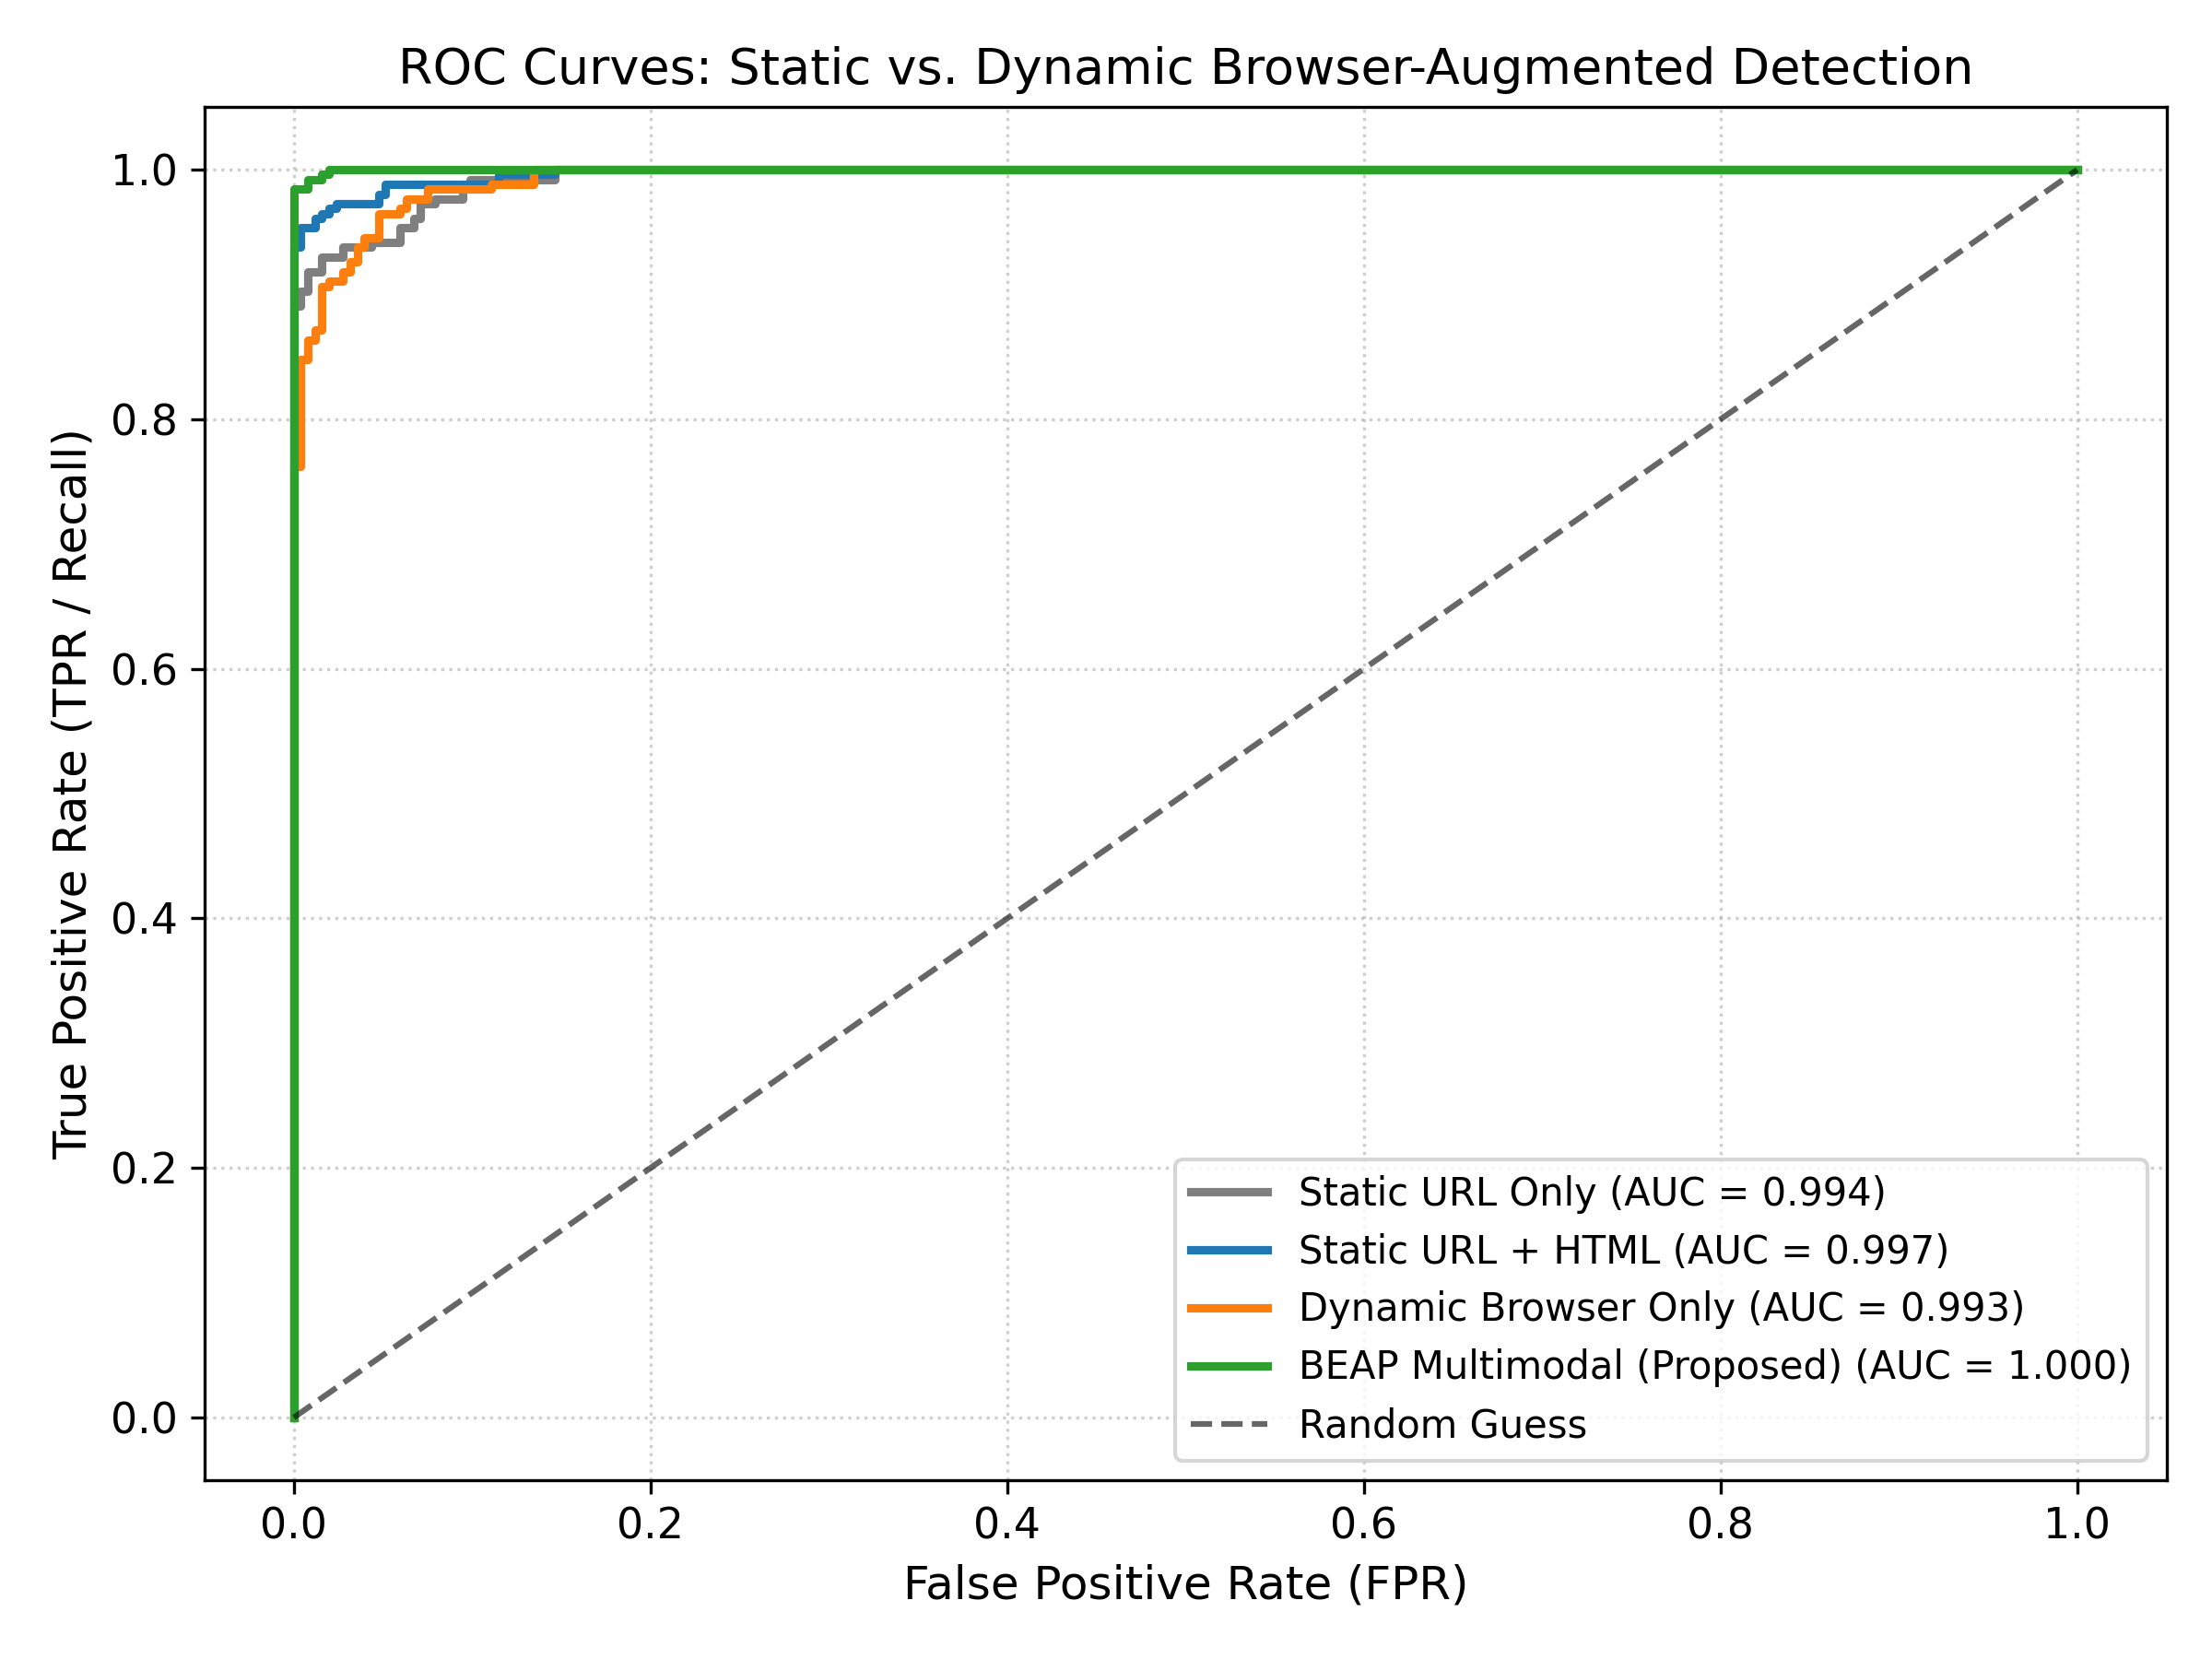
\includegraphics[width=0.46\textwidth]{figures/roc_curves.png}
\hfill
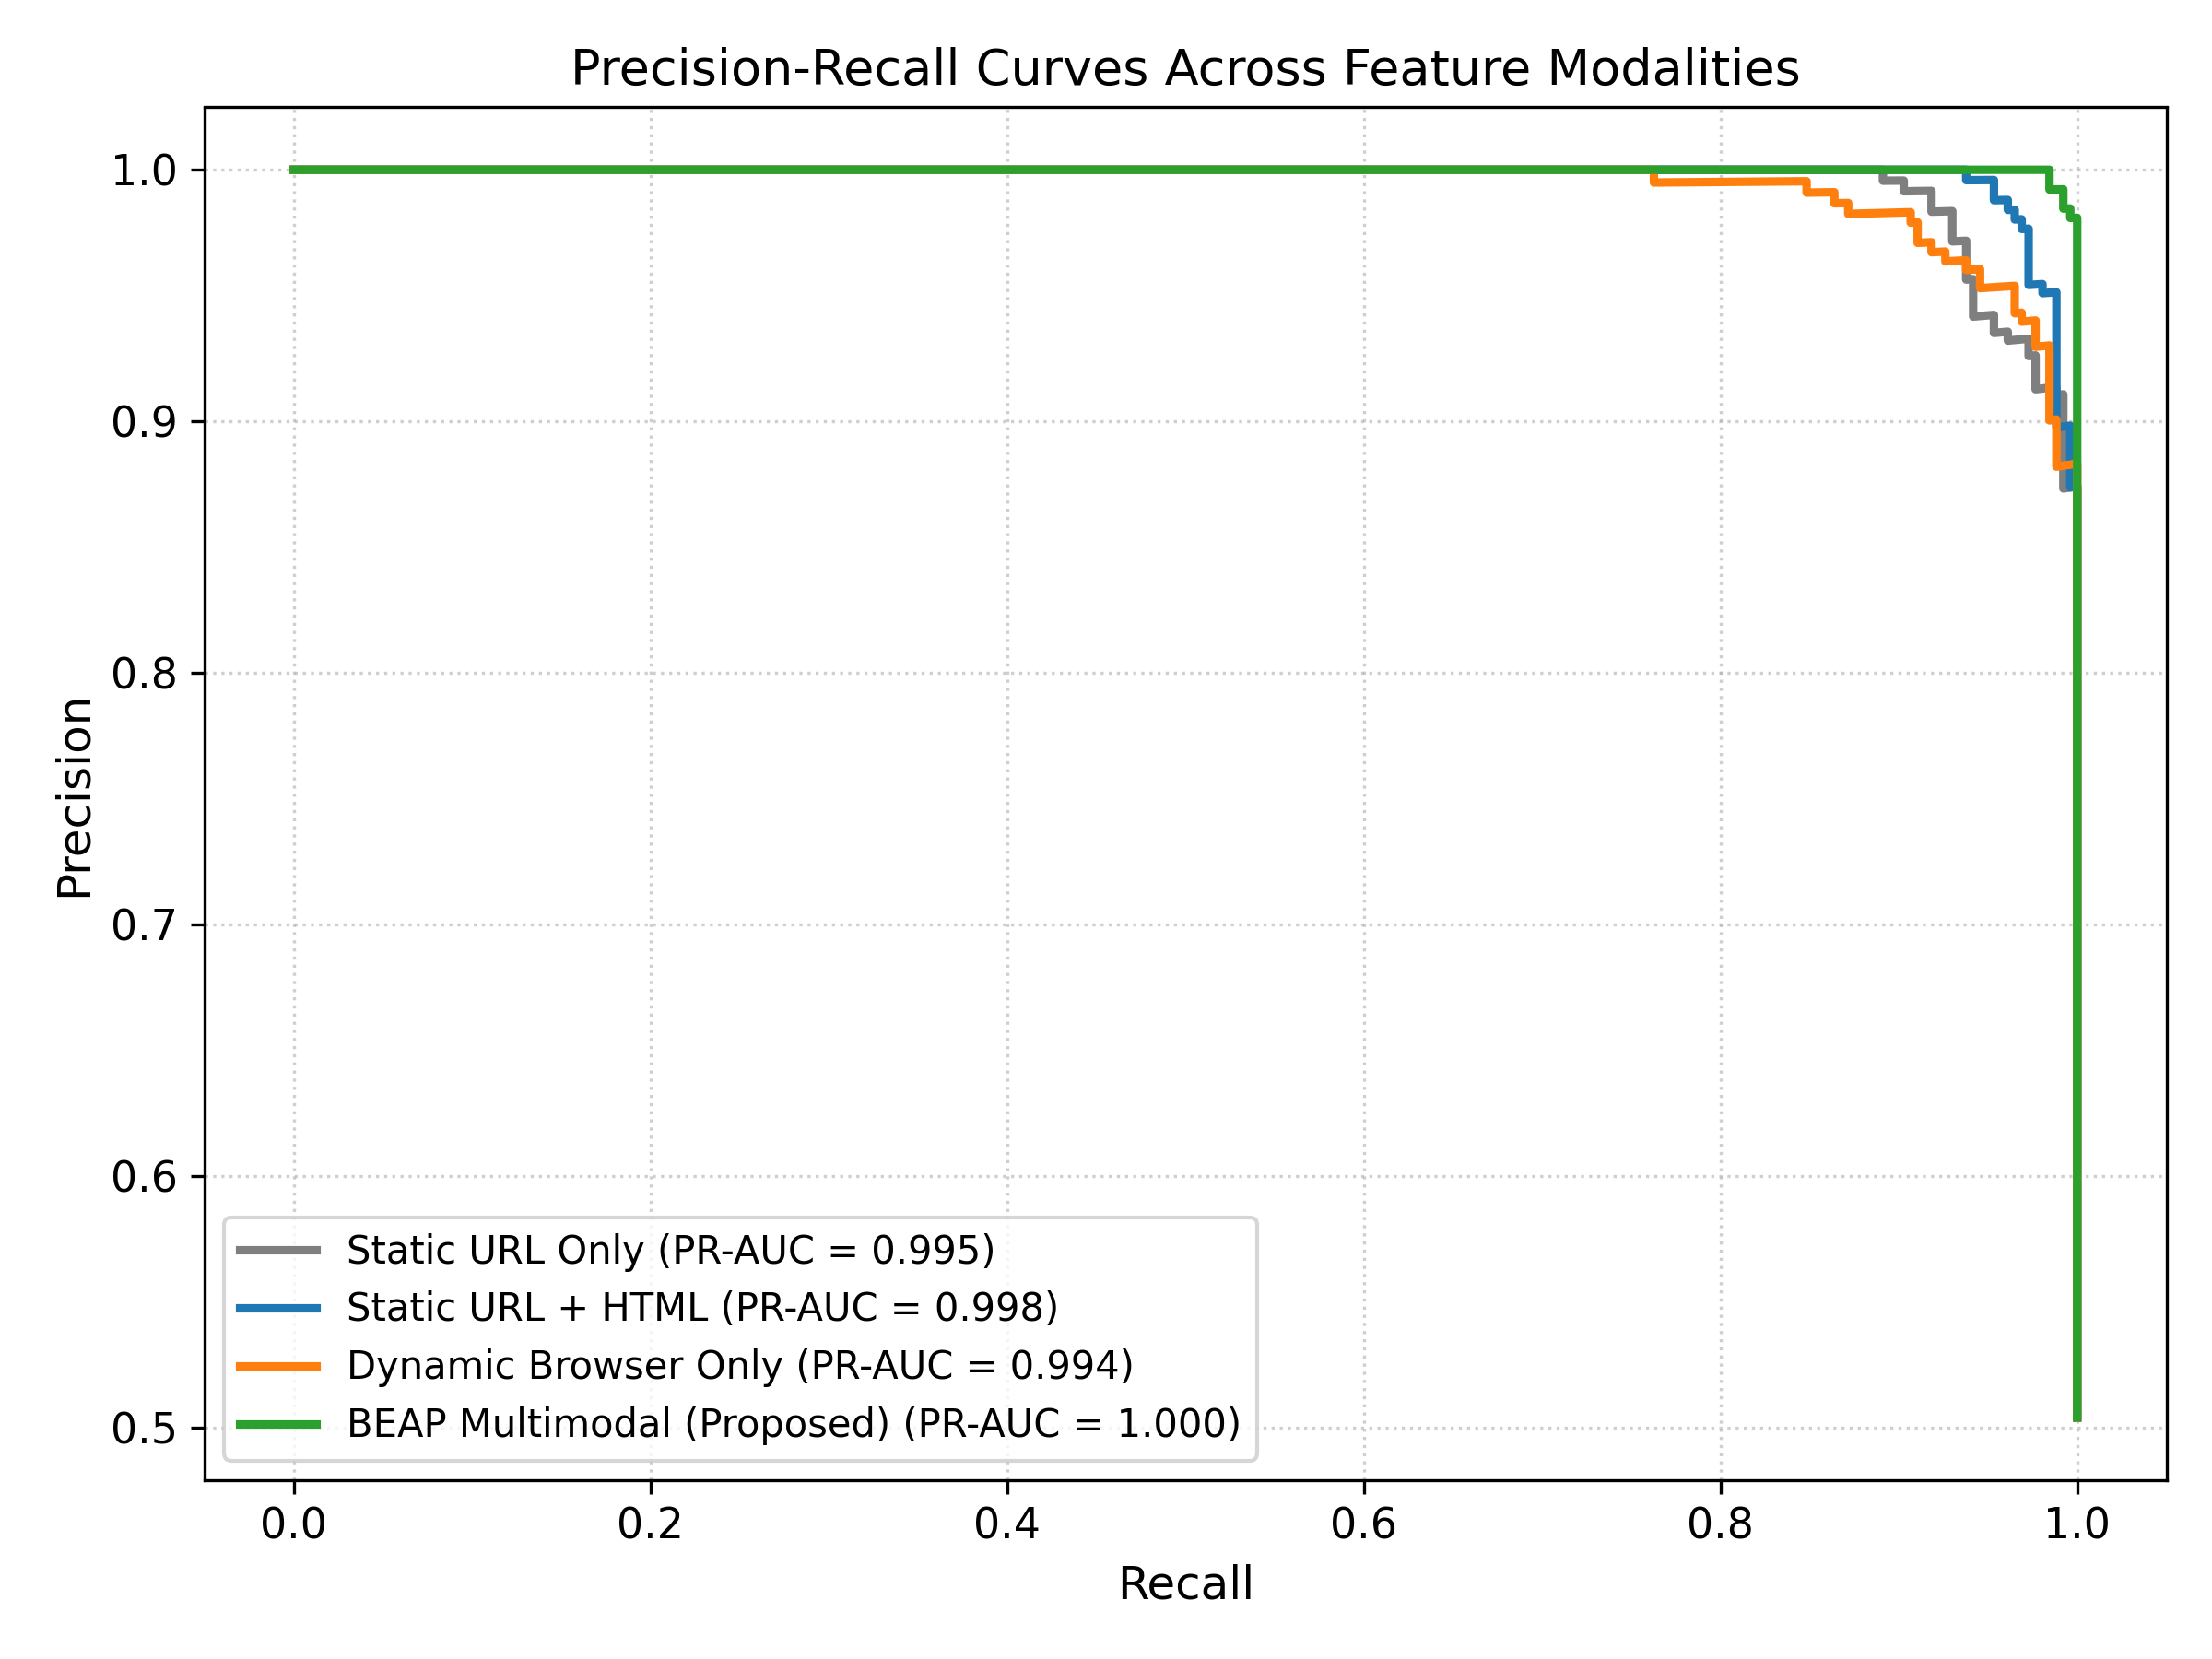
\includegraphics[width=0.46\textwidth]{figures/pr_curves.png}
\caption{ROC and PR curves across modalities under domain-disjoint evaluation.}
\label{fig:curves}
\end{figure}

Table~\ref{tab:ablation} and Fig.~\ref{fig:curves} report test results. Static URL features achieve 94.31\% accuracy, leaving 5.69\% error due to URL cloaking. Adding DOM features improves accuracy to 97.45\%. Dynamic evidence alone achieves 95.49\% accuracy. Integrating all signals in \textbf{BEAP Multimodal} delivers \textbf{99.22\% accuracy} (ROC-AUC 0.9998) for calibrated Logistic Regression and 99.41\% for XGBoost.

\begin{table}[t]
\caption{Detailed breakdown of key indicators across transport, behavioral, and lexical layers.}
\label{tab:features}
\centering
\setlength{\tabcolsep}{4pt}
\renewcommand{\arraystretch}{0.92}
\begin{tabular}{llccl}
\toprule
\textbf{Category} & \textbf{Feature Identifier} & \textbf{Weight} & \textbf{Impact} & \textbf{Operational Security Rationale} \\
\midrule
Security & \texttt{csp\_blocks\_eval\_inline} & $-1.8361$ & Trust ($-$) & Prohibits untrusted inline scripts and evaluation. \\
Headers  & \texttt{x\_frame\_options\_strict} & $-1.3075$ & Trust ($-$) & \texttt{DENY}/\texttt{SAMEORIGIN} blocks clickjacking framing. \\
         & \texttt{has\_hsts} & $-0.5205$ & Trust ($-$) & Enforces encrypted transport; prevents stripping. \\
         & \texttt{has\_x\_content\_type} & $-0.4812$ & Trust ($-$) & \texttt{nosniff} directive blocks MIME-confusion attacks. \\
\midrule
TLS \&   & \texttt{cert\_longevity\_days} & $-2.1606$ & Trust ($-$) & Long lifespans ($>180$\,d) typical of vetted orgs. \\
Certs    & \texttt{cert\_valid} & $-0.6876$ & Trust ($-$) & Cryptographic chain verifies basic authenticity. \\
         & \texttt{cert\_is\_free\_automated} & $-0.1771$ & Neutral & Short-lived CAs (Let's Encrypt); neutral alone. \\
\midrule
Behavior & \texttt{form\_action\_cross\_domain}& $+0.1711$ & Phish ($+$) & Forms transmitting data to foreign domains. \\
\& Forms & \texttt{has\_iframe} & $+1.3027$ & Phish ($+$) & Obfuscated frames embedding external forms. \\
         & \texttt{has\_sensitive\_input} & $+0.8415$ & Phish ($+$) & Password or credential harvesting fields. \\
\midrule
URL      & \texttt{suspicious\_keyword\_count}& $+2.7127$ & Phish ($+$) & Targeted tokens (\textit{login}, \textit{verify}, \textit{update}). \\
Lexical  & \texttt{hostname\_length} & $+1.3782$ & Phish ($+$) & Subdomain masking over reputable cloud hosts. \\
\bottomrule
\end{tabular}
\end{table}

\subsection{Indicator Analysis and Free TLS Certificate Disambiguation}

Table~\ref{tab:features} provides an individual analysis across feature families. HTTP security response headers serve as dominant trust anchors: strict CSP ($-1.8361$), clickjacking controls ($-1.3075$), HSTS ($-0.5205$), and MIME protections ($-0.4812$) deliver substantial negative log-odds attributions. Legitimate organizations invest in transport hardening, whereas disposable phishing deployments routinely omit these configurations.

\textbf{Free TLS Certificate Handling:} Because automated CAs (e.g., Let's Encrypt, ZeroSSL) secure millions of legitimate websites, flagging free certificates as inherently malicious drives severe false positive rates. In BEAP, \texttt{cert\_is\_free\_automated} carries a near-neutral coefficient ($-0.1771$). BEAP \textbf{never} penalizes a website solely for using an automated certificate, resolving ambiguity via cross-modal conjunction:
\begin{itemize}[leftmargin=1.5em]
    \item \textit{Benign Let's Encrypt site:} Legitimate forms route within origin ($x_{\text{cross}}=0$), and established security headers supply robust negative log-odds attributions that easily overcome certificate lifespan penalties.
    \item \textit{Phishing Let's Encrypt site:} Although encrypted by Let's Encrypt, forms exfiltrate credentials to foreign endpoints ($x_{\text{cross}}=1.0$), response headers are absent, and hostnames contain lexical anomalies. The alert triggers on behavioral exfiltration and omitted transport controls, not the certificate provider.
\end{itemize}

\subsection{RQ2: Selective Abstention and Error Suppression}

\begin{table}[t]
\caption{Selective classification across uncertainty margins $\delta$ on test split ($N=510$).}
\label{tab:abstention}
\centering
\setlength{\tabcolsep}{4pt}
\renewcommand{\arraystretch}{0.92}
\begin{tabular}{lrlrrrrrr}
\toprule
\textbf{Model} & $\mathbf{\delta}$ & \textbf{Interval} & \textbf{Coverage} & \textbf{Abstain} & \textbf{Sel. Acc.} & \textbf{Sel. Risk} & \textbf{Sel. FNR} \\
\midrule
Static Baseline & 0.00 & $[0.50, 0.50]$ & 100.00\% & 0.00\% & 97.45\% & 2.55\% & 3.89\% \\
BEAP Multimodal & 0.00 & $[0.50, 0.50]$ & 100.00\% & 0.00\% & 99.22\% & 0.78\% & 0.78\% \\
Static Baseline & 0.15 & $[0.35, 0.65]$ & 97.84\% & 2.16\% & 98.20\% & 1.80\% & 3.19\% \\
BEAP Multimodal & 0.15 & $[0.35, 0.65]$ & 98.63\% & 1.37\% & 99.60\% & 0.40\% & 0.79\% \\
\textbf{Static Baseline} & \textbf{0.25} & $[0.25, 0.75]$ & 93.92\% & 6.08\% & 99.16\% & 0.84\% & 1.22\% \\
\textbf{BEAP Multimodal} & \textbf{0.25} & $[0.25, 0.75]$ & \textbf{97.84\%} & \textbf{2.16\%} & \textbf{100.00\%} & \textbf{0.00\%} & \textbf{0.00\%} \\
BEAP Multimodal & 0.35 & $[0.15, 0.85]$ & 96.27\% & 3.73\% & 100.00\% & 0.00\% & 0.00\% \\
\bottomrule
\end{tabular}
\end{table}

\begin{figure}[t]
\centering
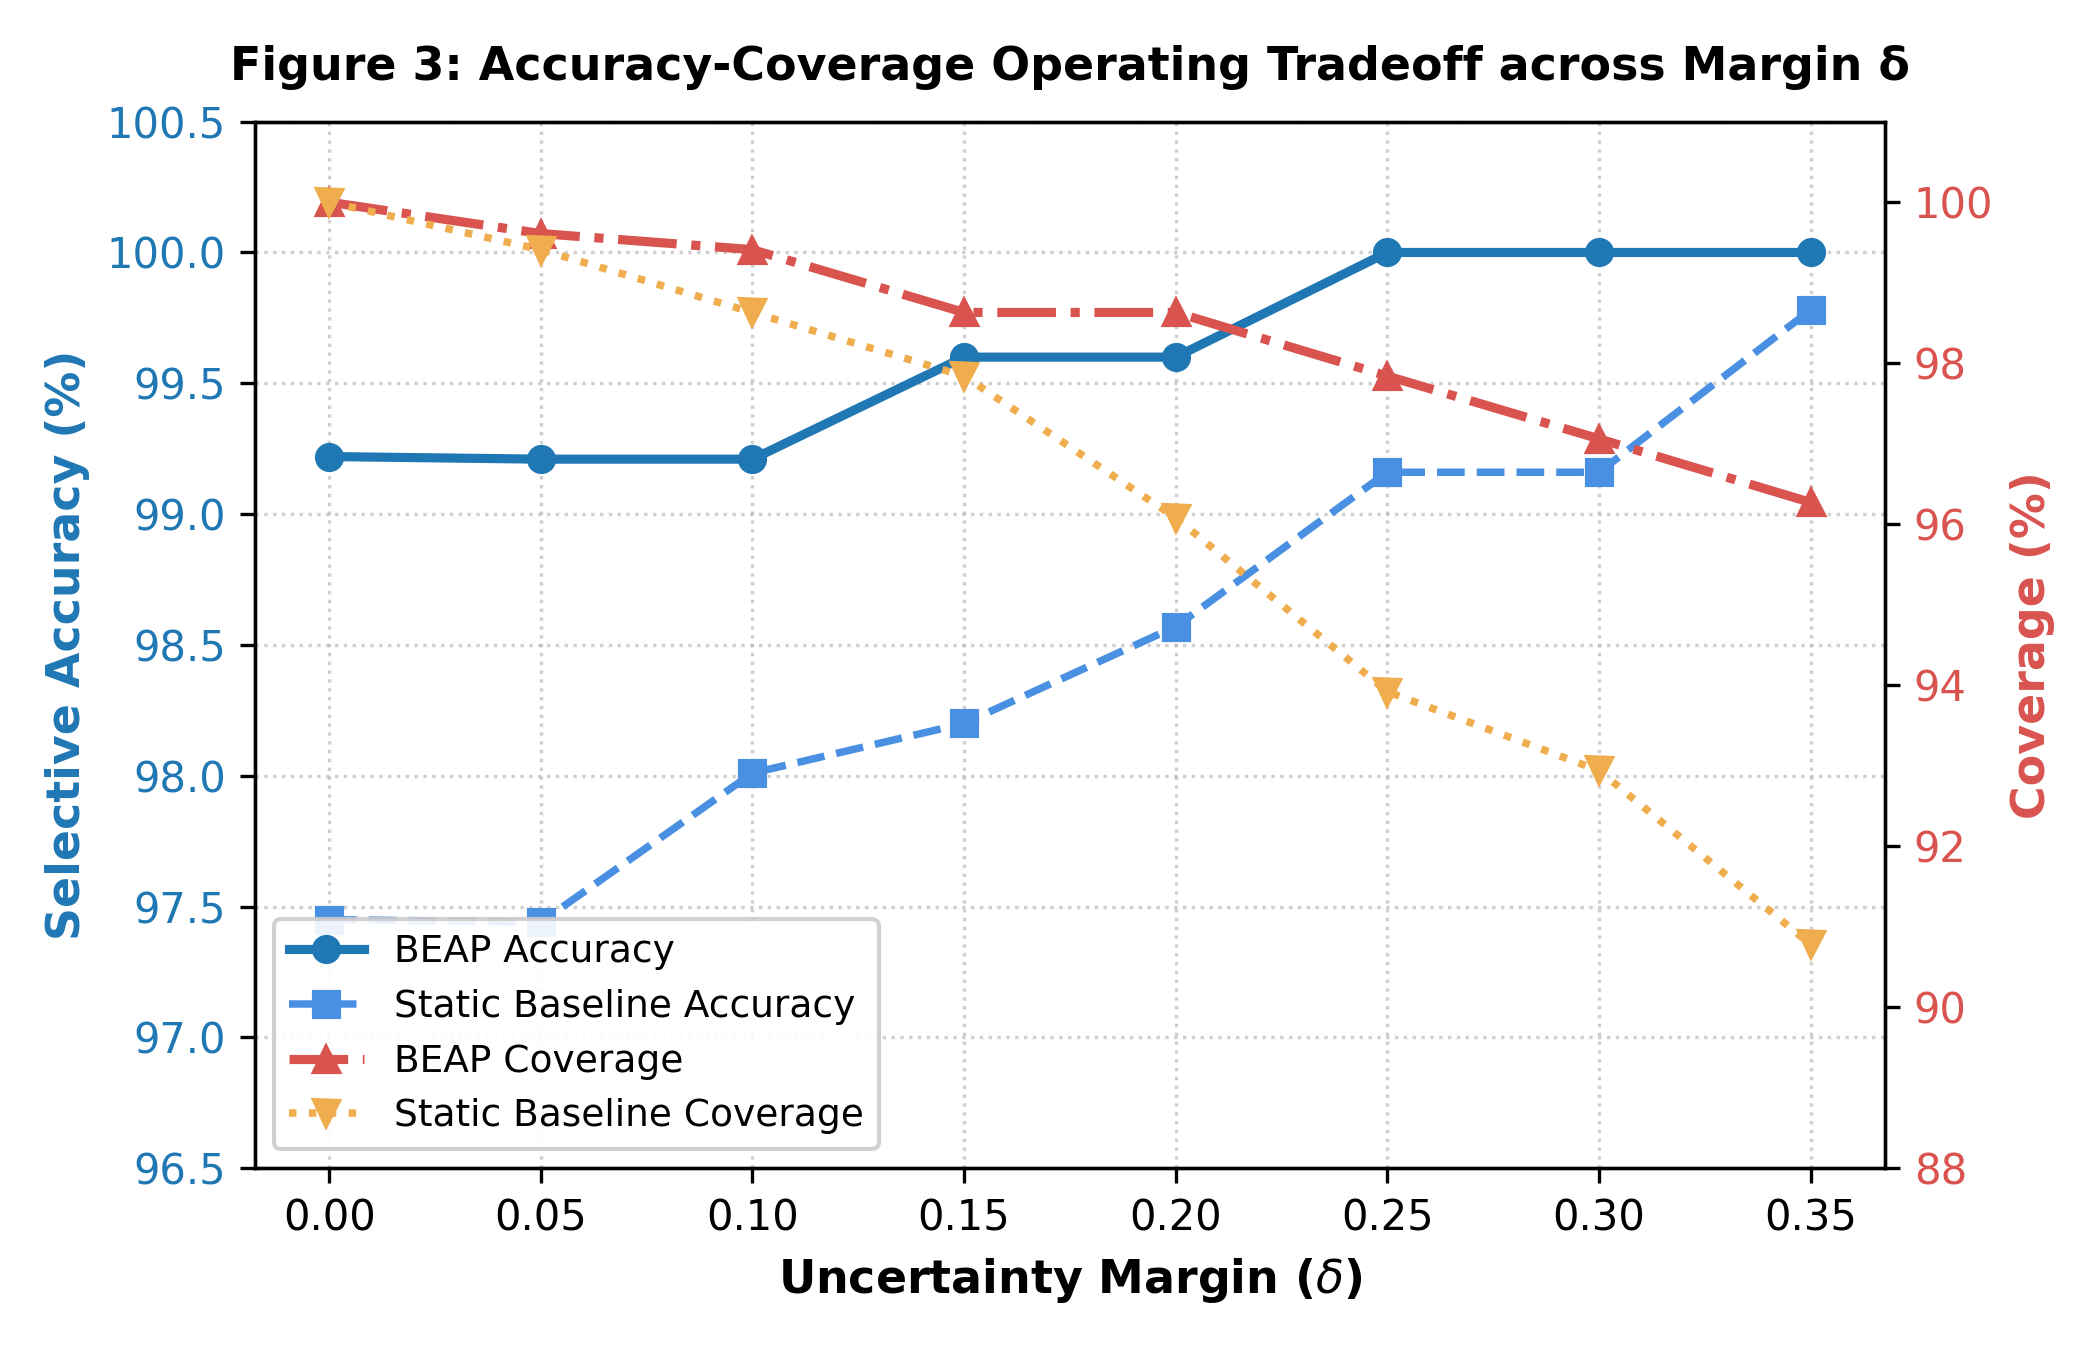
\includegraphics[width=0.46\textwidth]{figures/coverage_tradeoff.png}
\hfill
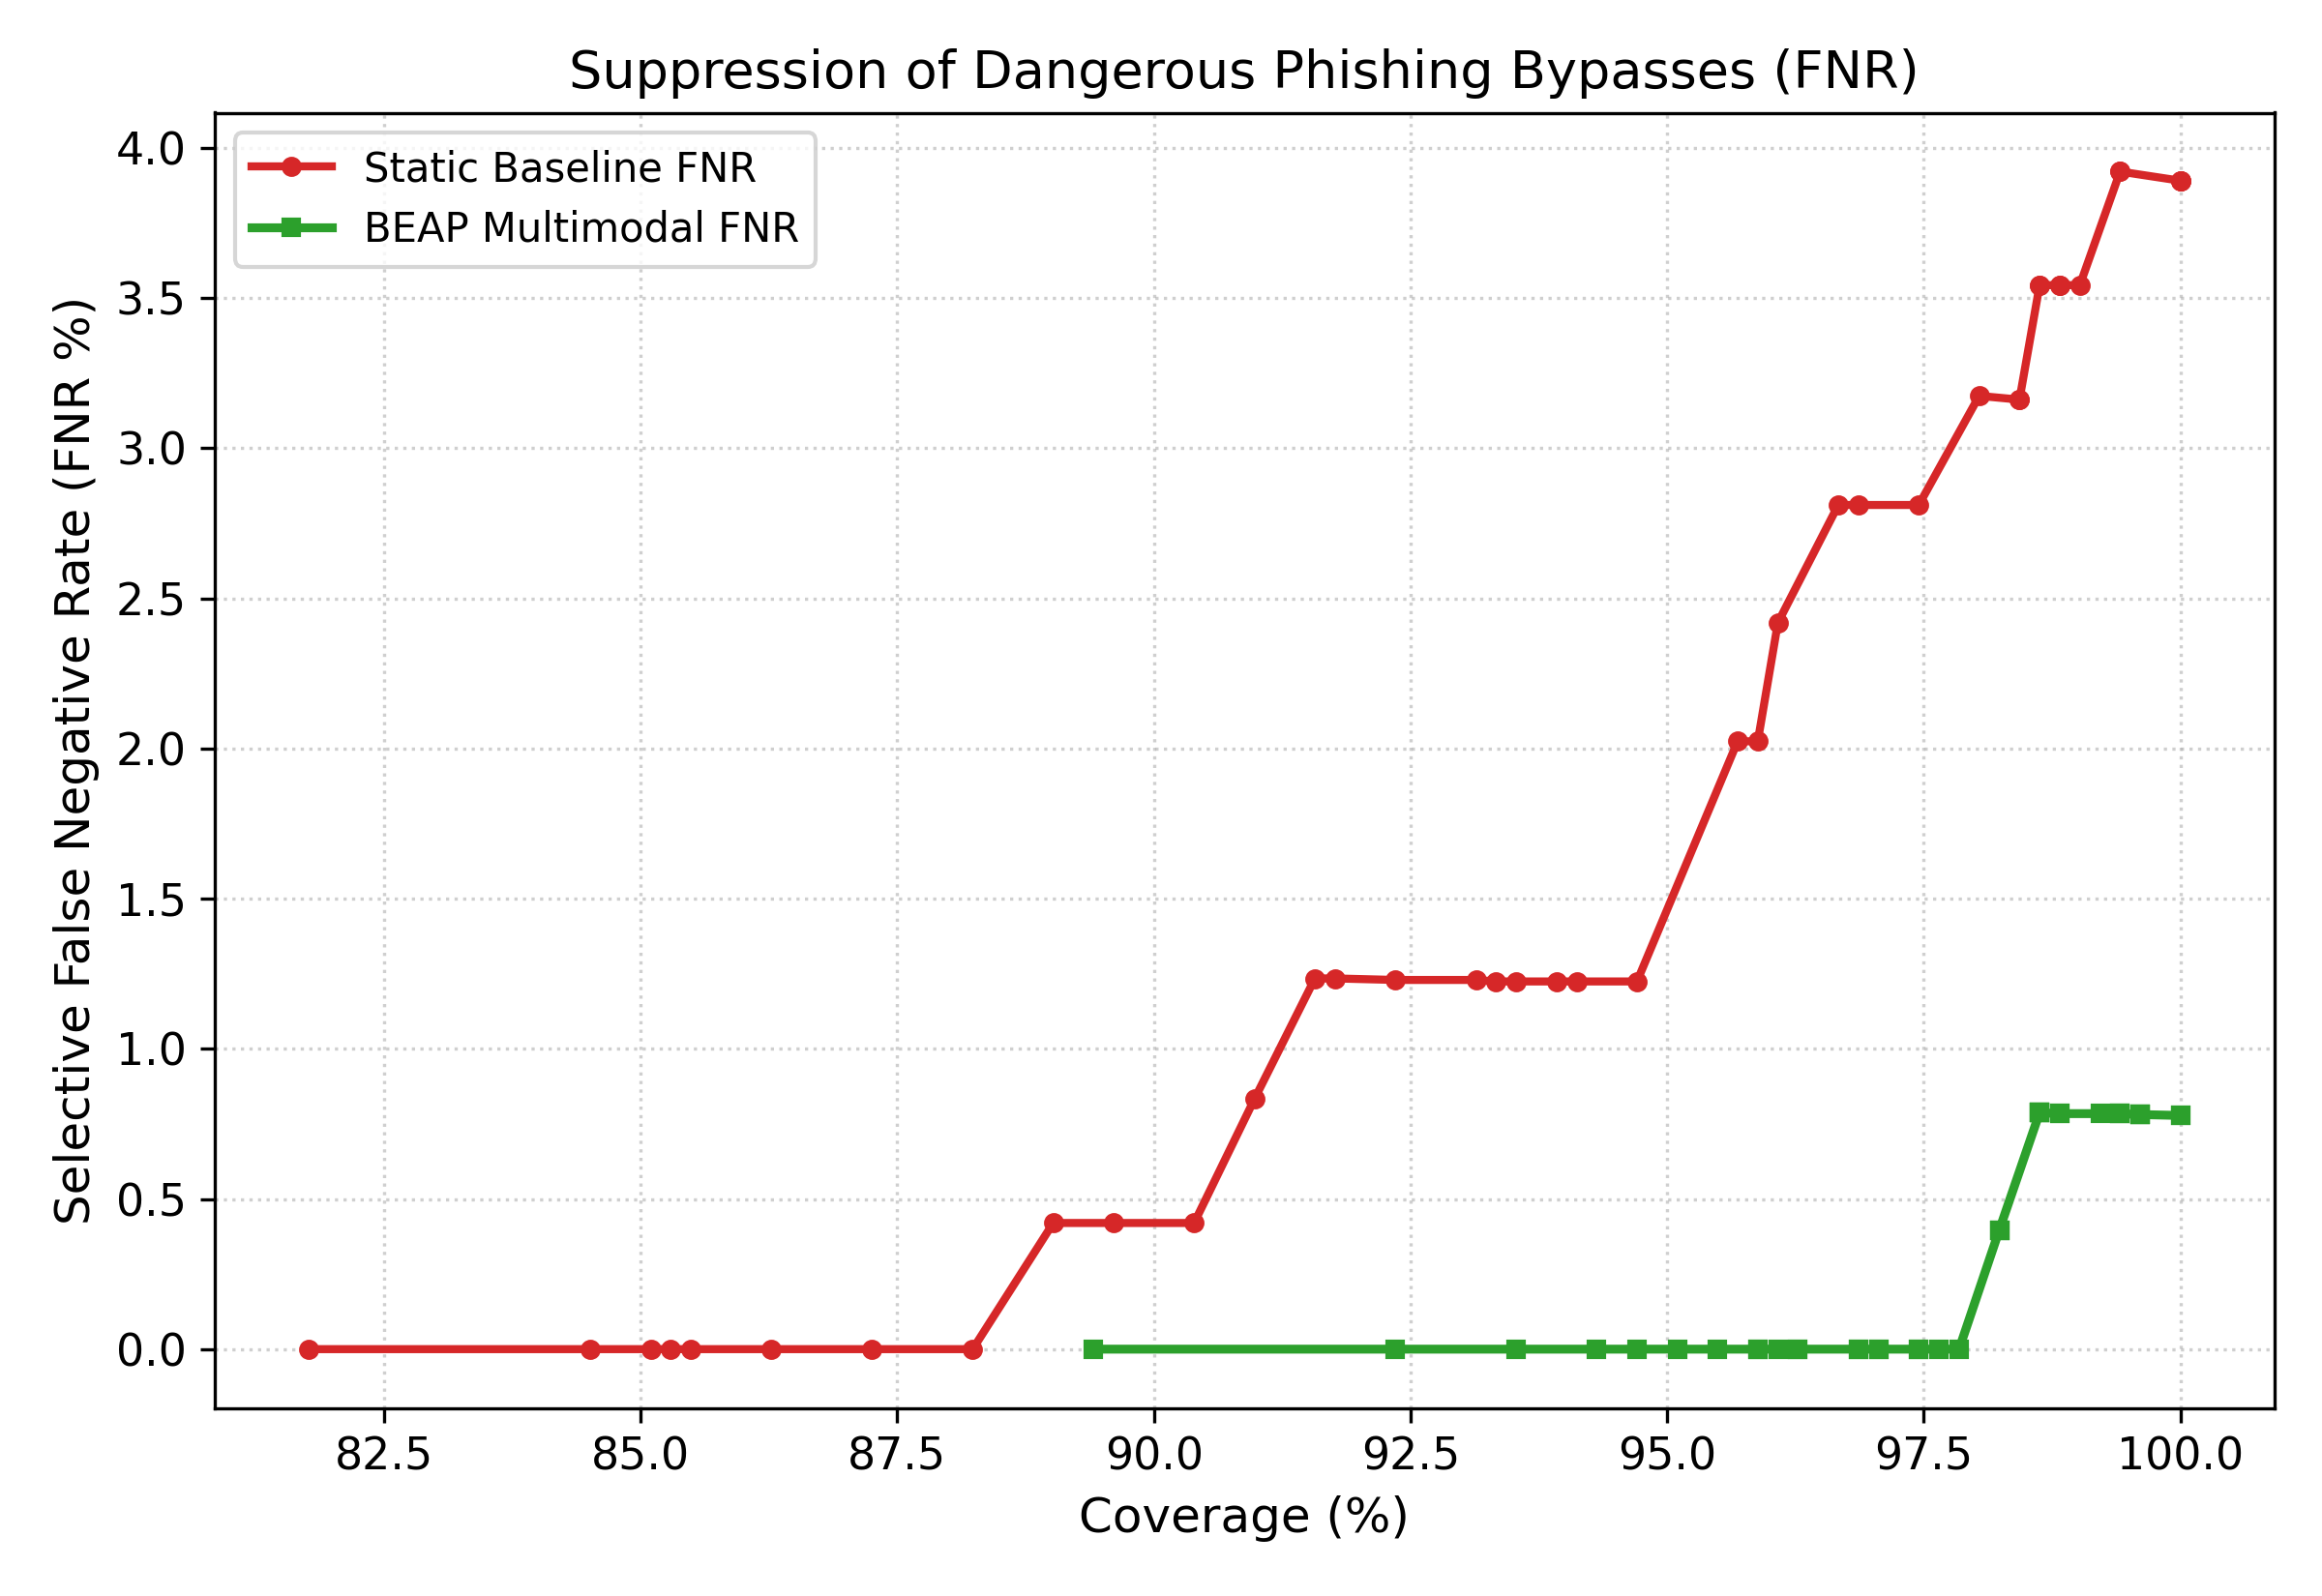
\includegraphics[width=0.46\textwidth]{figures/fnr_suppression_curve.png}
\caption{Coverage-accuracy trade-off and FNR suppression across abstention rate.}
\label{fig:abstention}
\end{figure}

Table~\ref{tab:abstention} and Fig.~\ref{fig:abstention} depict selective performance. At $\delta=0.00$, BEAP exhibits an initial FNR of 0.78\% and risk of 0.78\% (versus 3.89\% FNR and 2.55\% risk for static baseline). At $\delta=0.25$, abstaining on 2.16\% of borderline instances (11 cases) eliminates all observed test errors on covered traffic (97.84\% coverage). Residual risk naturally persists in open deployments; abstention functions as a practical operational filter rather than a theoretical perfection guarantee.

\subsection{RQ3: Performance Against Unseen Live Threat Intelligence Feeds}

Table~\ref{tab:feeds} evaluates BEAP on the 350 independent URLs from current threat intelligence feeds (OpenPhish, PhishTank). Without abstention ($\delta=0.00$), BEAP attains 98.86\% accuracy (Precision 0.9886, Recall 0.9886, F1 0.9886). Under selective abstention at $\delta=0.25$, BEAP abstains on 10 borderline instances (2.86\% abstention rate), achieving \textbf{99.71\% selective accuracy} and \textbf{0.00\% False Negative Rate (FNR)} over 97.14\% automated coverage. This confirms that dynamic transport indicators generalize effectively to active, in-the-wild zero-day campaigns.

\begin{table}[t]
\caption{Evaluation on independent live threat intelligence feed URLs ($N=350$).}
\label{tab:feeds}
\centering
\setlength{\tabcolsep}{5pt}
\renewcommand{\arraystretch}{0.92}
\begin{tabular}{lrrrrrr}
\toprule
\textbf{Evaluation Policy} & $\mathbf{\delta}$ & \textbf{Coverage} & \textbf{Abstain} & \textbf{Accuracy} & \textbf{Sel. Risk} & \textbf{Sel. FNR} \\
\midrule
Full Automation & 0.00 & 100.00\% & 0.00\% & 98.86\% & 1.14\% & 1.14\% \\
Moderate Abstention & 0.15 & 98.57\% & 1.43\% & 99.42\% & 0.58\% & 0.58\% \\
\textbf{High-Security Selective} & \textbf{0.25} & \textbf{97.14\%} & \textbf{2.86\%} & \textbf{99.71\%} & \textbf{0.29\%} & \textbf{0.00\%} \\
\bottomrule
\end{tabular}
\end{table}

\subsection{RQ4: Measured Latency and Efficiency}

\begin{table}[t]
\caption{Latency breakdown and literature benchmarking on single-core CPU.}
\label{tab:latency}
\centering
\setlength{\tabcolsep}{4.5pt}
\renewcommand{\arraystretch}{0.92}
\begin{tabular}{lllrr}
\toprule
\textbf{System / Architecture} & \textbf{Measurement Basis} & \textbf{Hardware} & \textbf{Latency} & \textbf{Throughput} \\
\midrule
Static Parsing (URL \& DOM) & Directly Measured & Single CPU Core & 0.40\,ms & 2,475\,eps \\
Dynamic Header \& Cert & Directly Measured & Single CPU Core & 0.65\,ms & 1,529\,eps \\
Scaling \& Vectorization & Directly Measured & Single CPU Core & 0.15\,ms & 6,711\,eps \\
Inference \& Log-Odds & Directly Measured & Single CPU Core & 0.24\,ms & 4,166\,eps \\
\textbf{BEAP Total Pipeline} & \textbf{Directly Measured} & \textbf{Single CPU Core} & \textbf{2.03\,ms} & \textbf{491.7\,eps} \\
BEAP (XGBoost + SHAP) & Directly Measured & Single CPU Core & 6.38\,ms & 156.7\,eps \\
Graph Fusion~\cite{kavya2025} & Reported in Literature & High-End GPU & 233.50\,ms & 4.28\,eps \\
Visual CNN~\cite{lin2021} & Reported in Literature & GPU / Server CPU & 372.00\,ms & 2.69\,eps \\
\bottomrule
\end{tabular}
\end{table}

Table~\ref{tab:latency} summarizes timing benchmarks over 1,000 runs. BEAP's computational decision pipeline executes in \textbf{2.03\,ms} on a single Intel CPU core (491.7 evaluations/sec) using $<25$\,MB RAM. This is $114\times$ faster than deep multimodal graph fusion (233.5\,ms)~\cite{kavya2025} without requiring GPU infrastructure.

\subsection{Case Study: Explainable Triage Walkthrough}

Consider an evasive PayPal lure (\url{https://auth-verification-paypal-notice.xyz/account/login}):
\begin{itemize}[leftmargin=1.5em]
    \item \textit{Static Assessment:} Standard form markup yields an ambiguous score ($p_{\text{static}} = 0.54$).
    \item \textit{Dynamic Assessment:} Active inspection reveals cross-domain form targets (\url{http://malicious-collector-hub.net/steal.php}), 45-day certificate longevity, and absent HSTS/CSP headers.
    \item \textit{Attribution:} Calibrated probability $p = 0.999 \ge \tau_{\text{high}}$ (Automated Block). Model decomposition details: \texttt{suspicious\_keyword\_count} ($+5.70$), \texttt{hostname\_length} ($+3.30$), \texttt{cert\_longevity} ($+1.75$), and \texttt{form\_action\_cross\_domain} ($+0.17$).
\end{itemize}

\section{Discussion and High-Volume Operational SOC Triage}

When deploying selective abstention in production environments, traffic spikes may overwhelm SOC triage capacity. To prevent review queues from saturating when analysts cannot inspect all deferred cases immediately, we propose four operational triage principles:
\begin{enumerate}[leftmargin=1.8em]
    \item \textbf{Directional Risk-Prioritized Queueing:} Deferred requests are ordered descending by posterior probability $f(\mathbf{x})$. Borderline high-risk instances ($p \approx 0.70$) surface ahead of borderline low-risk ambiguities ($p \approx 0.30$), maximizing analyst interception of evasive phishing.
    \item \textbf{Multi-Tier Severity Partitioning:} Requests featuring active password prompts and cross-domain action destinations are routed to Tier-1 emergency response. Ambiguous pages without credential prompts receive Tier-2 asynchronous inspection.
    \item \textbf{Safe Deferral Containment:} Deferred URLs are temporarily quarantined under Remote Browser Isolation (RBI) or read-only credential masking rather than defaulting to open access, preventing credential exfiltration during triage delays.
    \item \textbf{Dynamic Margin Modulation:} Under acute queue overflow, the uncertainty margin $\delta$ can be dynamically tightened from 0.25 to 0.15, increasing automated throughput to 98.63\% while preserving 99.60\% accuracy.
\end{enumerate}

\section{Threats to Validity and Limitations}

\begin{enumerate}[leftmargin=1.8em]
    \item \textbf{Processing vs. Network Probing Latency:} A distinction separates BEAP's 2.03\,ms algorithmic pipeline from network transport latency (0.5--2.0\,s). BEAP mitigates transport overhead via an exponential-decay LRU domain cache ($T_{1/2} = 24$\,h).
    \item \textbf{Dynamic Cloaking:} Sophisticated adversaries may inspect client fingerprints and withhold malicious content~\cite{lin2021}, requiring stealth browser automation profiles.
    \item \textbf{Adversarial Adaptation:} Adversaries may purchase aged domains or configure basic security headers to mimic legitimate infrastructure, which BEAP combats through cross-modal joint evidence.
\end{enumerate}

\section{Conclusion and Reproducibility}

BEAP combines static lexical analysis, browser-observed dynamic evidence, and selective classification within an SSRF-safe execution boundary. Evaluating 2,400 samples across 1,379 unique domains under strict domain-disjoint partitioning demonstrates 99.22\% accuracy (ROC-AUC 0.9998) without abstention, and zero observed test errors at 97.84\% coverage ($\delta=0.25$). On 350 independent live threat intelligence feed URLs, BEAP achieves 99.71\% selective accuracy with zero false negatives. Executing in 2.03\,ms on a single CPU core, BEAP delivers an auditable, high-throughput defense. Reproduction code, benchmark data, and the inspection dashboard are available at: \url{https://github.com/mitesh-k/beap-phishing-detection}.

\begin{thebibliography}{22}

\bibitem{basit2021}
Basit, A., Zafar, M., Liu, X., Javed, A.R., Jalil, Z., Kifayat, K.: A comprehensive survey of AI-enabled phishing attacks detection techniques. Telecommun. Syst. 76, 139--154 (2021)

\bibitem{tang2021}
Tang, L., Mahmoud, Q.H.: A survey of machine learning-based solutions for phishing website detection. Mach. Learn. Knowl. Extr. 3(3), 672--694 (2021)

\bibitem{zienie2023}
Zieni, R., Massari, L., Calzarossa, M.C.: Phishing or not phishing? A survey on the detection of phishing websites. IEEE Access 11, 18499--18519 (2023)

\bibitem{lin2021}
Lin, Y., Liu, R., Divakaran, D.M., Ng, J.Y., Chan, Q.Z., Lu, Y., Si, Y., Zhang, F., Dong, J.S.: Phishpedia: A hybrid deep learning based approach to visually identify phishing webpages. In: 30th USENIX Security Symposium, pp. 3793--3810 (2021)

\bibitem{anupam2021}
Anupam, S., Kar, A.K.: Phishing website detection using support vector machines and nature-inspired optimization algorithms. Telecommun. Syst. 76, 17--32 (2021)

\bibitem{bu2021}
Bu, S.-J., Cho, S.-B.: Deep character-level anomaly detection based on a convolutional autoencoder for zero-day phishing URL detection. Electronics 10(12), 1492 (2021)

\bibitem{purwanto2022}
Purwanto, R.W., Pal, A., Blair, A., Jha, S.: PhishSim: Aiding phishing website detection with a feature-free tool. IEEE Trans. Inf. Forensics Secur. 17, 1497--1512 (2022)

\bibitem{ariyadasa2022}
Ariyadasa, S., Fernando, S., Fernando, S.: Combining long-term recurrent convolutional and graph convolutional networks to detect phishing sites using URL and HTML. IEEE Access 10, 82355--82375 (2022)

\bibitem{sanchez2022}
S{\'a}nchez-Paniagua, M., Fern{\'a}ndez, E.F., Alegre, E., Al-Nabki, W., Gonz{\'a}lez-Castro, V.: Phishing URL detection: A real-case scenario through login URLs. IEEE Access 10, 42949--42960 (2022)

\bibitem{kara2022}
Kara, I., Ok, M., Ozaday, A.: Characteristics of understanding URLs and domain names features: The detection of phishing websites with machine learning methods. IEEE Access 10, 124420--124428 (2022)

\bibitem{chai2022}
Chai, Y., Zhou, Y., Li, W., Jiang, Y.: An explainable multi-modal hierarchical attention model for developing phishing threat intelligence. IEEE Trans. Dependable Secur. Comput. 19, 790--803 (2022)

\bibitem{kalabarige2023}
Kalabarige, L.R., Rao, R.S., Pais, A.R., Gabralla, L.A.: A boosting-based hybrid feature selection and multi-layer stacked ensemble learning model to detect phishing websites. IEEE Access 11, 71180--71193 (2023)

\bibitem{castano2023}
Casta{\~n}o, F., Fern{\'a}ndez, E.F., Alaiz-Rodr{\'i}guez, R., Alegre, E.: PhiKitA: Phishing kit attacks dataset for phishing websites identification. IEEE Access 11, 40779--40789 (2023)

\bibitem{zhao2023}
Almousa, M., Anwar, M.: A URL-based social semantic attacks detection with character-aware language model. IEEE Access 11, 10654--10663 (2023)

\bibitem{alsubaei2024}
Alsubaei, F.S., Almazroi, A.A., Ayub, N.: Enhancing phishing detection: A novel hybrid deep learning framework for cybercrime forensics. IEEE Access 12, 8373--8389 (2024)

\bibitem{reyes2024}
Reyes-Dorta, N., Caballero-Gil, P., Rosa-Remedios, C.: Detection of malicious URLs using machine learning. Wirel. Netw. 30, 7543--7560 (2024)

\bibitem{calzarossa2025}
Calzarossa, M.C., Giudici, P., Zieni, R.: An assessment framework for explainable AI with applications to cybersecurity. Artif. Intell. Rev. 58, 150 (2025)

\bibitem{kavya2025}
Kavya, S., Sumathi, D.: Multimodal and temporal graph fusion framework for advanced phishing website detection. IEEE Access 13, 74128--74146 (2025)

\bibitem{shukla2024}
Shukla, S., Misra, M., Varshney, G.: HTTP header based phishing attack detection using machine learning. Trans. Emerg. Telecommun. Technol. 35(1), e4872 (2024)

\bibitem{hendrickx2024}
Hendrickx, K., Perini, L., Van der Plas, D., Meert, W., Davis, J.: Machine learning with a reject option: A survey. Mach. Learn. 113, 3073--3110 (2024)

\bibitem{kustiawan2025}
Kustiawan, Y.A., Ghauth, K.I.: Feature engineering for phishing website detection using machine learning: A systematic review. IEEE Access 13, 192080--192104 (2025)

\bibitem{vaddempudi2025}
Vaddempudi, N.S., Sajja, D., Phanidar, C., Basavaraju, S.: Lightweight and explainable phishing URL detection using feature selection and XGBoost. In: Proc. IIPEM, pp. 1--6 (2025)

\end{thebibliography}

\end{document}